In Data Center history we witnessed a shift towards smaller devices used
as client actors inside our systems: with the advent of cloud computing and
mobile devices, portability and scalability are being able to further develop
inside our applications. Also, it's easier to update the data inside a shared
and cloud connected database instead to update millions of devices around the
world, users have ease of management (with little configurations needed) and
many application services can run at a low cost per user: it is worth noting 
that many application require the strength, power and availability of a
full datacenter to perform some specific workloads (see search engines).
\begin{figure}[H]
    \centering
    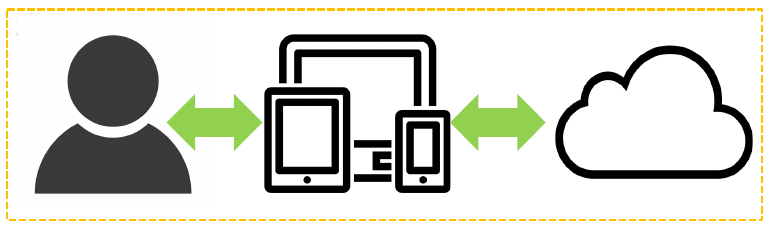
\includegraphics[width=0.7\textwidth]{Images/4SmallerClients}
    \caption{Distributed Software}
\end{figure} 

\subsection{From Data Centers to Warehouse-Scale Computers...}
This trend created a new class of computing systems that needed to emerge from
regular datacenters whose main characteristic was to have lots of power to 
host a large number of small-medium sized applications, each one running on 
dedicated hardware and isolated with software for multiple organizations. 
\textbf{WSC} are made for single organizations, where the hardware is relatively 
homogeneous and applications have a common system manager layer and talk to 
each other: it can be considered as a large cluster of servers that needs to 
be considered as a single computing unit. It is meant to run a smaller number
of very large applications. 
\begin{key}{Warehouse-Scale Computers}
    \textbf{WSC} are large scale datacenters accomunated by homogeneous hardware
    and are to be considered a single computational unit made by a single 
    organization for the developement of multiple large-scale applications.
\end{key}
\begin{figure}[H]
    \centering
    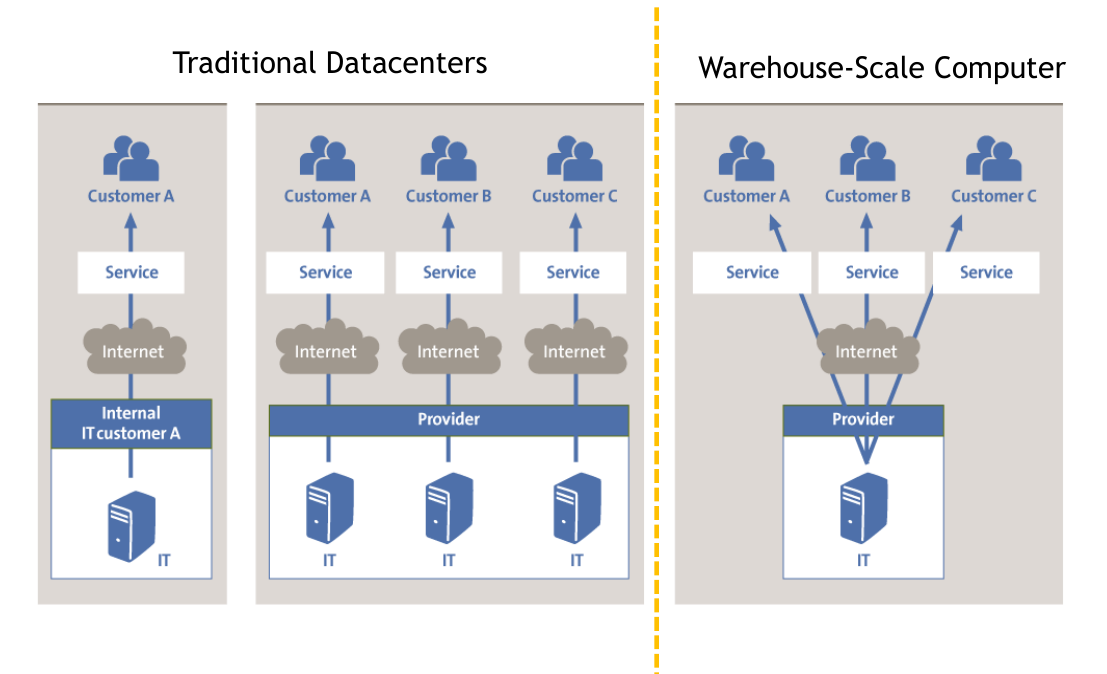
\includegraphics[width=0.9\textwidth]{Images/5WSCvsDatacenters.png}
    \caption{Traditional Data Center vs WSC}
\end{figure}
\subsection{...and Back}
Right now, Amazon, Microsoft and Google are all using this model for their
public clouds computing systems, but in a more traditional-oriented way: since
such public clouds use lots of little applications, they are operated like a 
datacenter thanks to virtualization inside the system. WSC implements the 
traditional paradigm thanks to Virtual Machines.
\begin{figure}[H]
    \centering
    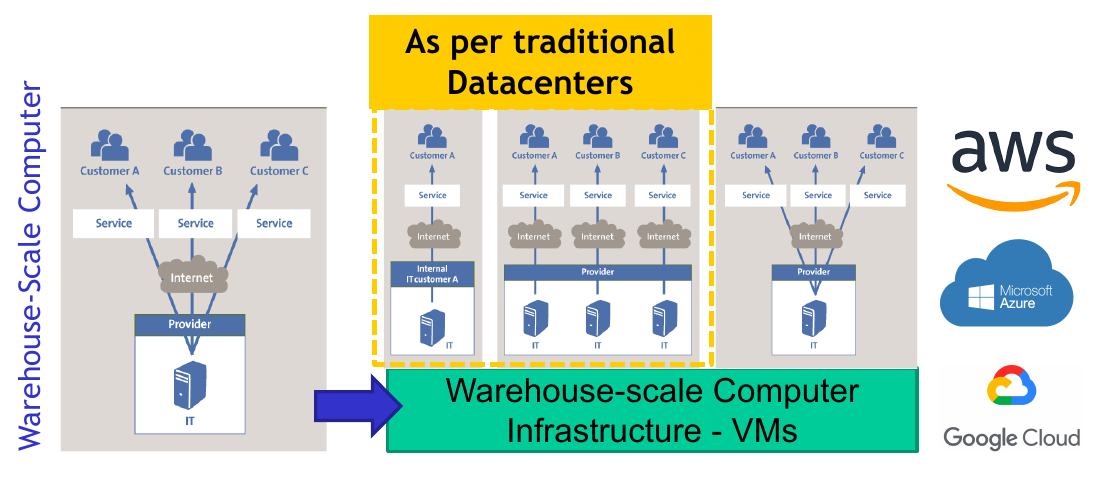
\includegraphics[width=0.9\textwidth]{Images/6WSCVirtual.png}
    \caption{WSC with Virtualization}
\end{figure}
\begin{notice}{DataCenter Replicas}
    Even if single requests are typically processed by a single datacenter, it 
    is good practice to replicate the same datacenter to reduce latency and 
    improve throughput.
\end{notice}
\subsection{Areas and Regions}
To be sure that all the users are served it is possible to use different 
approaches:
\begin{itemize}
    \item \textbf{Geographic Areas (GAs)} - we can use geopolitical boundaries
    to better distribute the loads and to grant data residency: it is mandatory
    that in the same GA there are at least two computing regions
    \item \textbf{Computer Regions (CRs)} - a finer grain of location: it is 
    confined by latency (<2ms), distance (<100 miles apart) and disaster 
    recovery.
    \item \textbf{Availability Zones (AZs)} - a finer grain of location within a
    single \textbf{CR}: multiple DC in a single CR allows to run mission 
    critical applications,  syncronicity of data is granted by a 
    quorum of minimum three data centers.  
\end{itemize}
\begin{figure}[H]
    \centering
    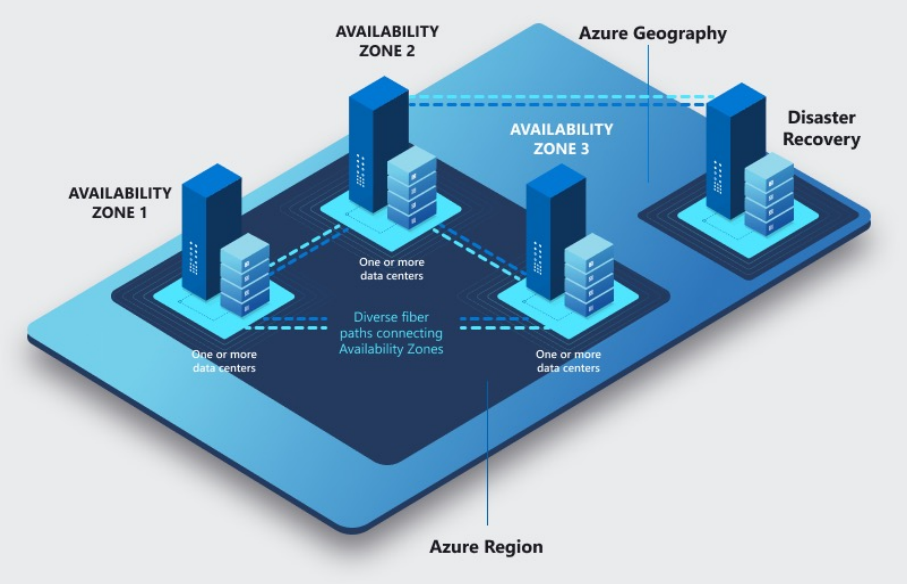
\includegraphics[width=0.8\textwidth]{Images/7Azure.png}
    \caption{Azure Architecture inside a \textbf{GA}}
\end{figure}

\subsubsection{Edge DataCenters}
To satisfy latency and to grant coverage in all areas, sometimes companies
use \textbf{Edge DataCenters}, smaller datacenters made exclusively to filter
requests that were going to the main datacenters. Sometimes, companies prefer
to have many Edge DataCenters that serve a single main DataCenter.
\begin{figure}[H]
    \centering
    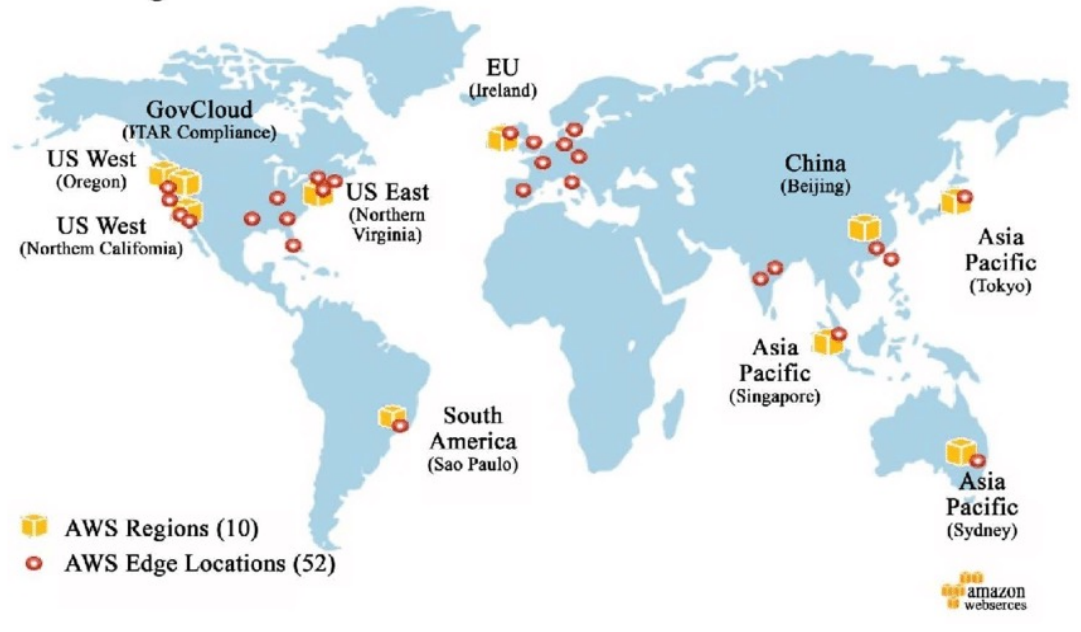
\includegraphics[width=0.8\textwidth]{Images/8EdgeDC.png}
    \caption{Map of Amazon AWS Edge DataCenters with relative 
    Main DataCenters}
\end{figure}

\subsubsection{Availability and Uptime}
Usually Uptime is pretty high among those type of datacenters:
\begin{itemize}
    \item \textbf{Single Instance VMs} - 99.90\%
    \item \textbf{Availability Sets} - 99.95\%
    \item \textbf{Availability Zones} - 99.99\%
 \end{itemize}

 \subsection{Architectural Overview of WSCs}
 \begin{figure}[H]
    \centering
    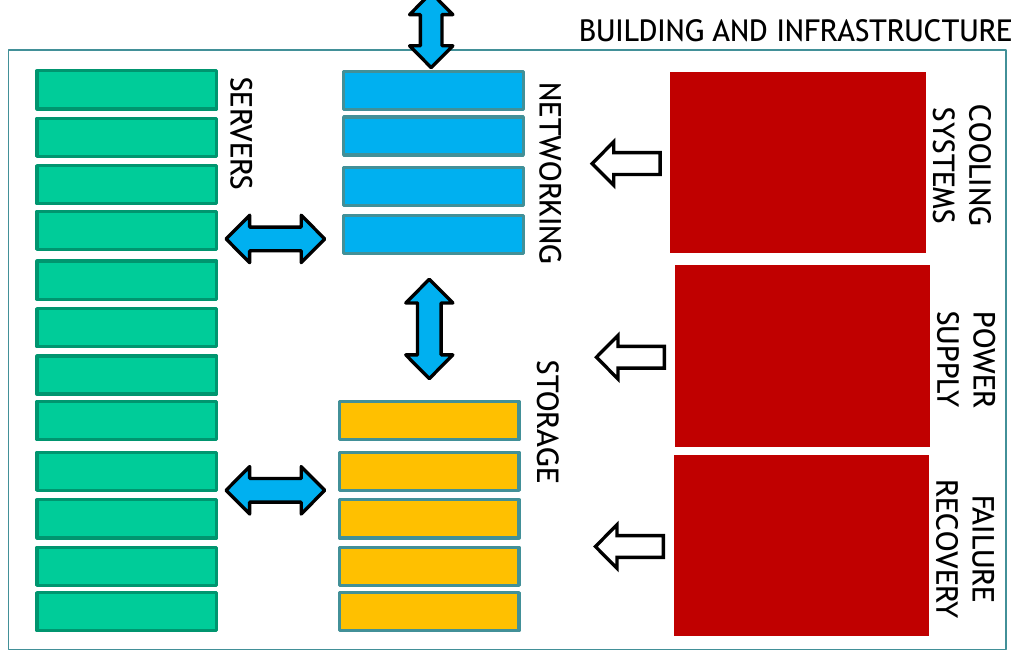
\includegraphics[width=0.8\textwidth]{Images/9WSCArchitecture.png}
    \caption{WSC General Architecture}
\end{figure}

\begin{itemize}
    \item \textbf{Servers and Rack} - the main processing equipement, hosted
    inside shelves as basic building blocks of DC and WSC, connected by 
    hirarchies of network.
    \item \textbf{Storage} - the backbone of the system, composed in different
    ways depending on the necessities (\textbf{DAS}, \textbf{NAS}, 
    \textbf{SAN}, \textbf{RAID}).
    \item \textbf{Networking} - also called \textbf{DCN} (DataCenter Network), connects
    every component of the system with switches, routers, load balancers and
    cables.
    \item \textbf{Power, Cooling and Failure Recovery} - all the necessary to 
    maintain the whole infrastructure solid and working.
\end{itemize}
